\section{Design}
\label{sec:Design}

\subsection{How Are You Going to Build It?}
For the development of LinkedGym, we embraced a user-centric approach, focusing on how and who the product will benefit. This strategy involved several stages to ensure we understood the exact needs of the user and integrated these insights into our design. To build LinkedGym, we adopted the Agile methodology, with a particular focus on the Scrum framework. Agile's iterative and incremental development process is ideal for our project, allowing us to adapt swiftly to changing requirements and deliver value consistently. Here's an overview of our initial phase and the development process:

\begin{enumerate}
  \item \textbf{Identifying User Needs and Benefits:} We started with establishing who the major users of LinkedGym would be—fitness coaches and trainees. Our goal was to provide a unified solution which aims to provide improved solutions for the coaching services, as well as to ensure smooth training process of the trainees.
  
  \item \textbf{Brainstorming and Concept Development:} Using brainstorming techniques like Crazy 8s, we generated a wide array of ideas. We then combined the best concepts to create user stories and personas, which helped us visualize our target users and their needs.
  
  \item \textbf{User Journey Mapping and Testing:} We evolved these insights into detailed user journey maps and performed user testing sessions to gather feedback. This process ensured that our design effectively addressed user pain points and preferences.
  
  \item \textbf{Prototyping:} We divided the application into two parts for optimal convenience: a web app for coaches and a mobile app for trainees. Using Figma, we developed prototypes and performed multiple rounds of user testing, refining the prototypes based on the feedback received.
\end{enumerate}

\subsection{Architecture}
We planned LinkedGym's architecture to support scalability, flexibility, and a seamless user experience across both the web and mobile platforms. The key components of our architecture include:

\subsubsection{Frontend:}
\begin{itemize}
  \item \textbf{Web Application:} Would be developed using modern web technologies such as React or Angular, ensuring a responsive and interactive interface for coaches.
  
  \item \textbf{Mobile Application:} Built using Flutter or React Native would deliver a consistent user experience on both iOS and Android for trainees.
\end{itemize}

\subsubsection{Backend:}
\begin{itemize}
  \item \textbf{Firebase Integration:} We chose to utilize Firebase for its comprehensive suite of tools, including Realtime Database, Cloud Firestore, Authentication, Cloud Functions, and Hosting, to streamline development and ensure high performance.
  
  \item \textbf{APIs:} Implementing RESTful APIs to facilitate efficient communication between the frontend and backend components, ensuring modularity and ease of maintenance.
  
  \item \textbf{Security:} Employing Firebase Authentication to provide secure and seamless user login and registration processes, safeguarding user data and privacy.
\end{itemize}

\subsection{Sketches, Storyboard, Wireframes/Prototype}
Our design process involved creating detailed sketches, storyboards, wireframes, and prototypes to visualize and iterate on the user experience. Key design elements included:

\subsubsection{User Personas and Stories}
Detailed personas and user stories helped us understand our target audience and their specific needs, guiding our design decisions.
\begin{figure}[H]
    \centering
    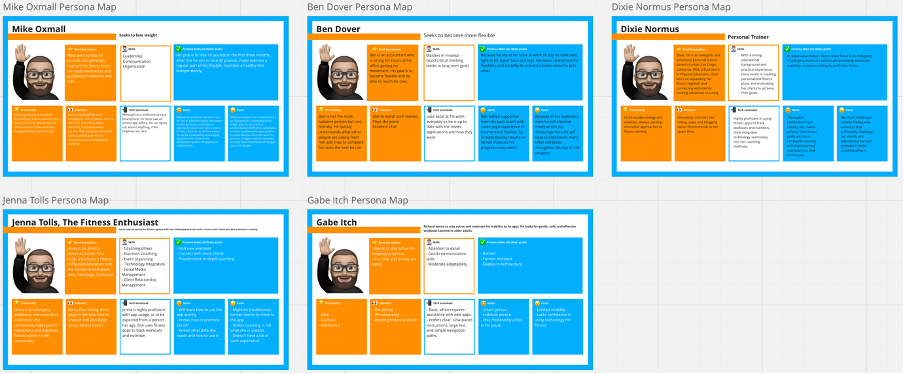
\includegraphics[width=0.8\textwidth]{images/personas.png}
    \caption{Persons}
    \label{fig:example_image}
  \end{figure}


\begin{itemize}
  \item \textbf{User Personas:} We created personas representing different types of users, including fitness coaches and trainees, to empathize with their goals, behaviors, and pain points.
  
  \item \textbf{User Stories:} We developed user stories to capture the requirements and expectations of each persona, ensuring that our design addressed real user needs.
\end{itemize}


\subsubsection{User Journey Maps}
Mapping the user journey allowed us to identify key interaction points and areas for improvement.

\begin{figure}[H]
    \centering
    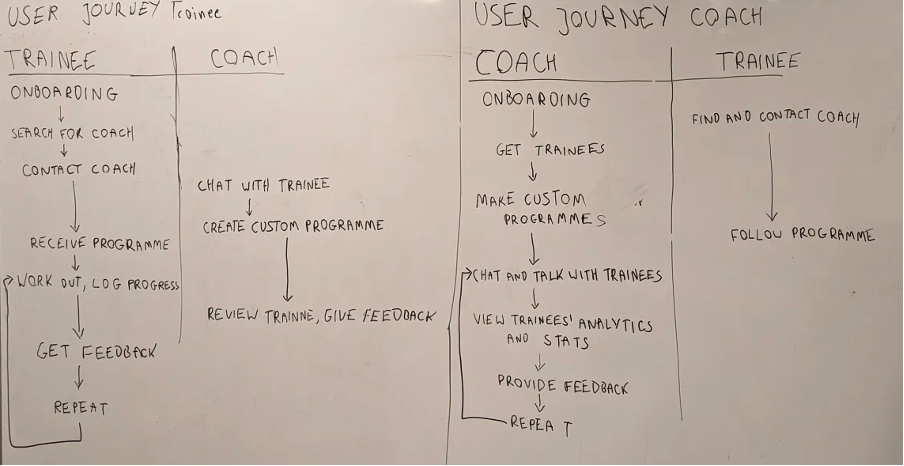
\includegraphics[width=0.8\textwidth]{images/userjourney.png}
    \caption{User Jouerney Map}
    \label{fig:userjourney}
  \end{figure}


\begin{itemize}
  \item \textbf{Mapping Process:} We visualized the user journey from initial interaction with the app to achieving their fitness goals, identifying touchpoints, emotions, and pain points along the way.
  
  \item \textbf{Feedback Incorporation:} Through user testing and feedback, we refined the user journey maps to ensure a smooth and intuitive experience for users.
\end{itemize}

\subsubsection{Wireframes and Prototypes}
Using Figma, we developed interactive prototypes for both the web and mobile applications. These prototypes were refined based on user testing feedback to ensure an optimal user experience.

\begin{figure}[H]
    \centering
    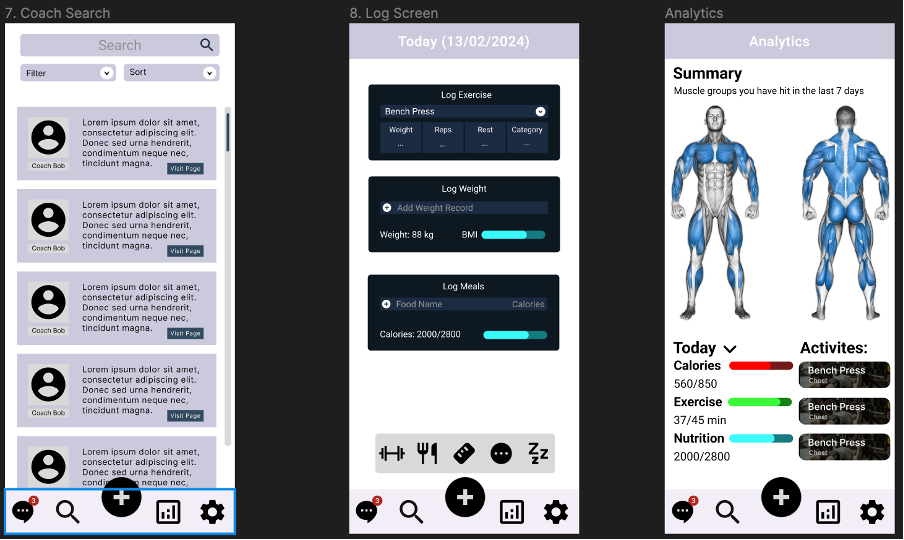
\includegraphics[width=0.8\textwidth]{images/figma.png}
    \caption{Mobile Application}
    \label{fig:figma}
  \end{figure}

  \begin{figure}[H]
    \centering
    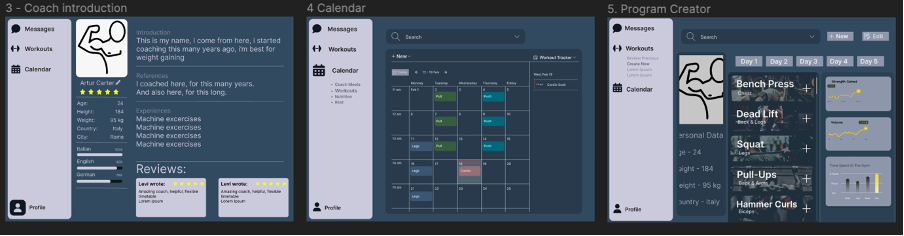
\includegraphics[width=0.8\textwidth]{images/figma2.png}
    \caption{Web Application}
    \label{fig:figma2}
  \end{figure}


\begin{itemize}
  \item \textbf{Wireframes:} We created wireframes to outline the layout and functionality of each screen in the application, focusing on usability and navigation.
  
  \item \textbf{Prototypes:} Interactive prototypes were developed to simulate user interactions and gather feedback on features such as navigation, content placement, and user flow.
\end{itemize}

\subsubsection{Detailed Design}
After finalizing the prototypes, we created UML diagrams, data models, and acceptance criteria. We also developed CRC cards, class diagrams, use case diagrams, sequence diagrams, state machine diagrams, RAID diagrams, and performed MoSCoW and SWOT analyses to ensure a robust and comprehensive design.

\begin{itemize}
  \item \textbf{UML Diagrams:} We used UML diagrams to visualize the structure and behavior of the system, including class diagrams, sequence diagrams, and state machine diagrams.
  
  \item \textbf{Data Models:} Data models were designed to represent the entities and relationships within the application, ensuring efficient data storage and retrieval.
  
  \item \textbf{Acceptance Criteria:} Clear acceptance criteria were defined to validate the functionality of the system and ensure that it met the requirements of stakeholders.
\end{itemize}

\begin{figure}[H]
    \centering
    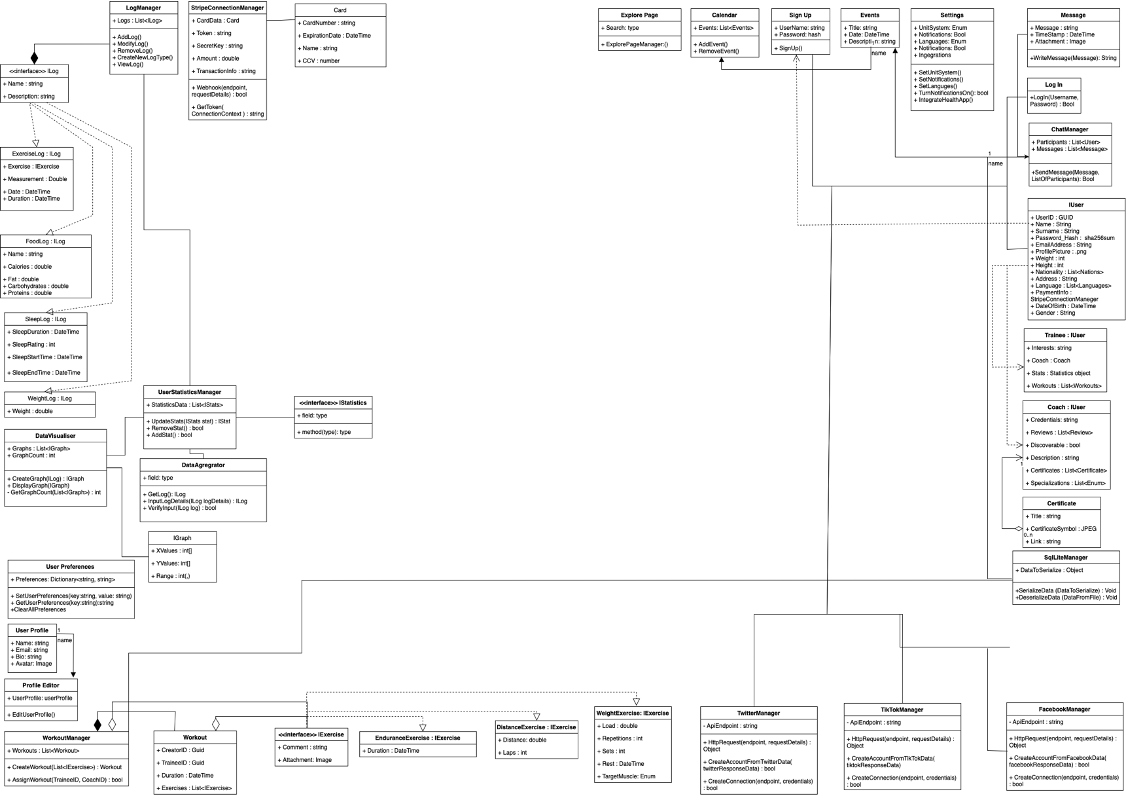
\includegraphics[width=0.8\textwidth]{images/crc.png}
    \caption{CRC Diagram}
    \label{fig:example_icrcmage}
  \end{figure}


\begin{figure}[H]
    \centering
    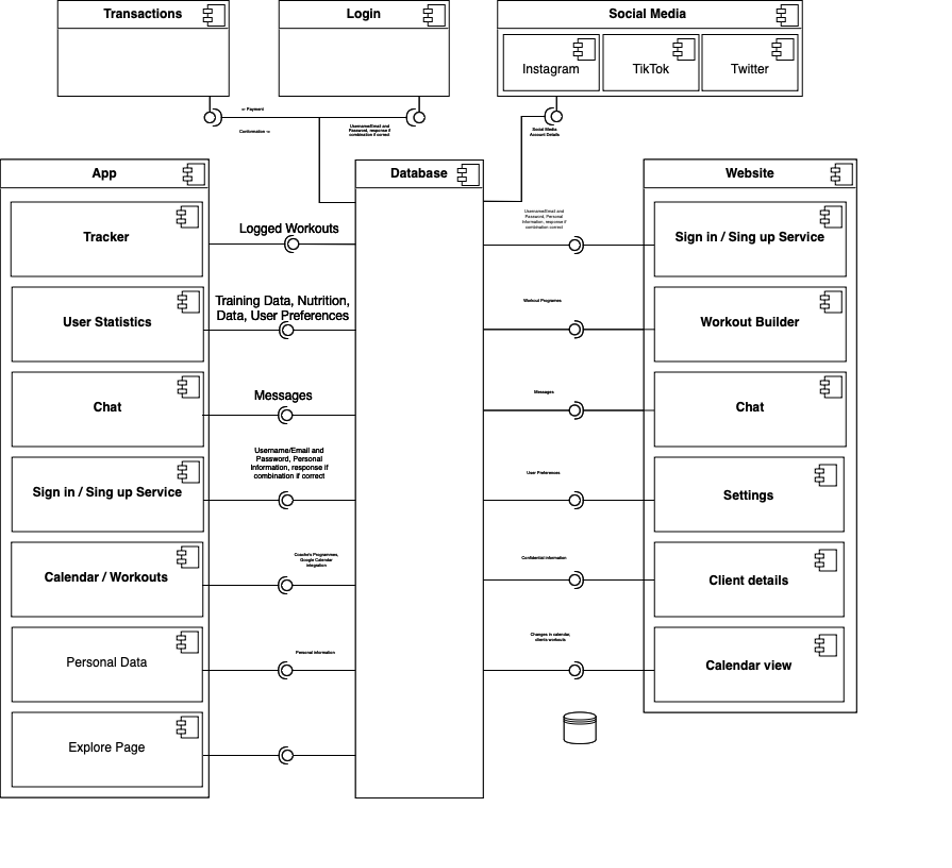
\includegraphics[width=0.8\textwidth]{images/uml.png}
    \caption{Database Structure}
    \label{fig:uml}
  \end{figure}

\begin{figure}[H]
    \centering
    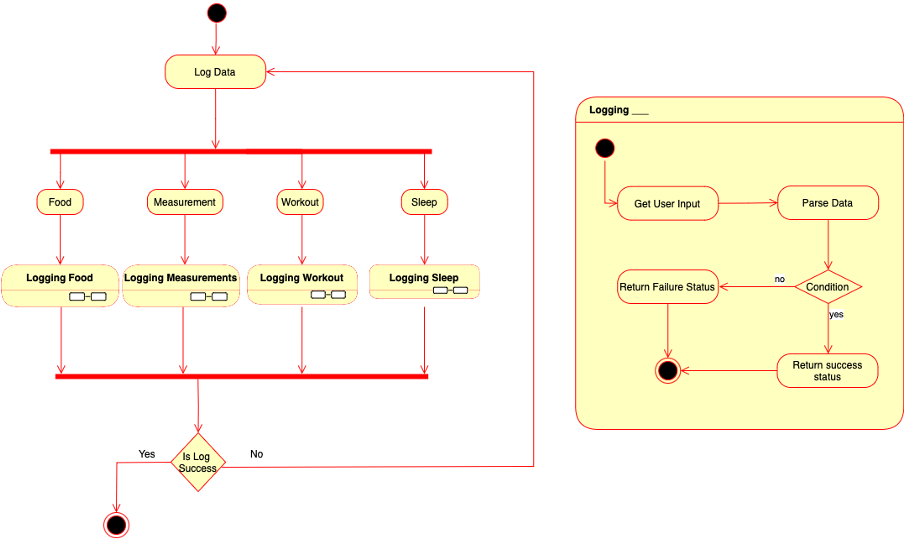
\includegraphics[width=0.8\textwidth]{images/state_machine.png}
    
    \caption{State Machine}
    \label{fig:state_machine}
  \end{figure}

 \begin{figure}[H]
    \centering
    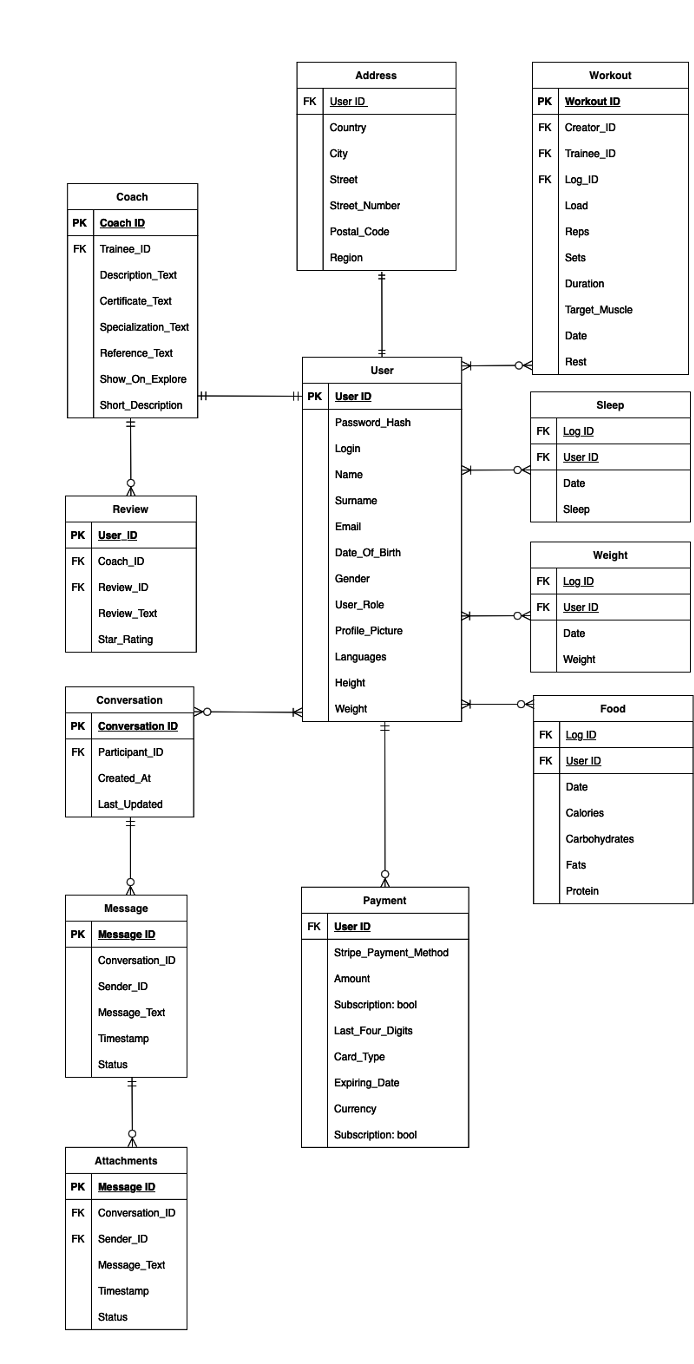
\includegraphics[width=0.8\textwidth]{images/uml2.png}
    \caption{ User Data }
    \label{fig:uml2}
  \end{figure}

   \begin{figure}[H]
    \centering
    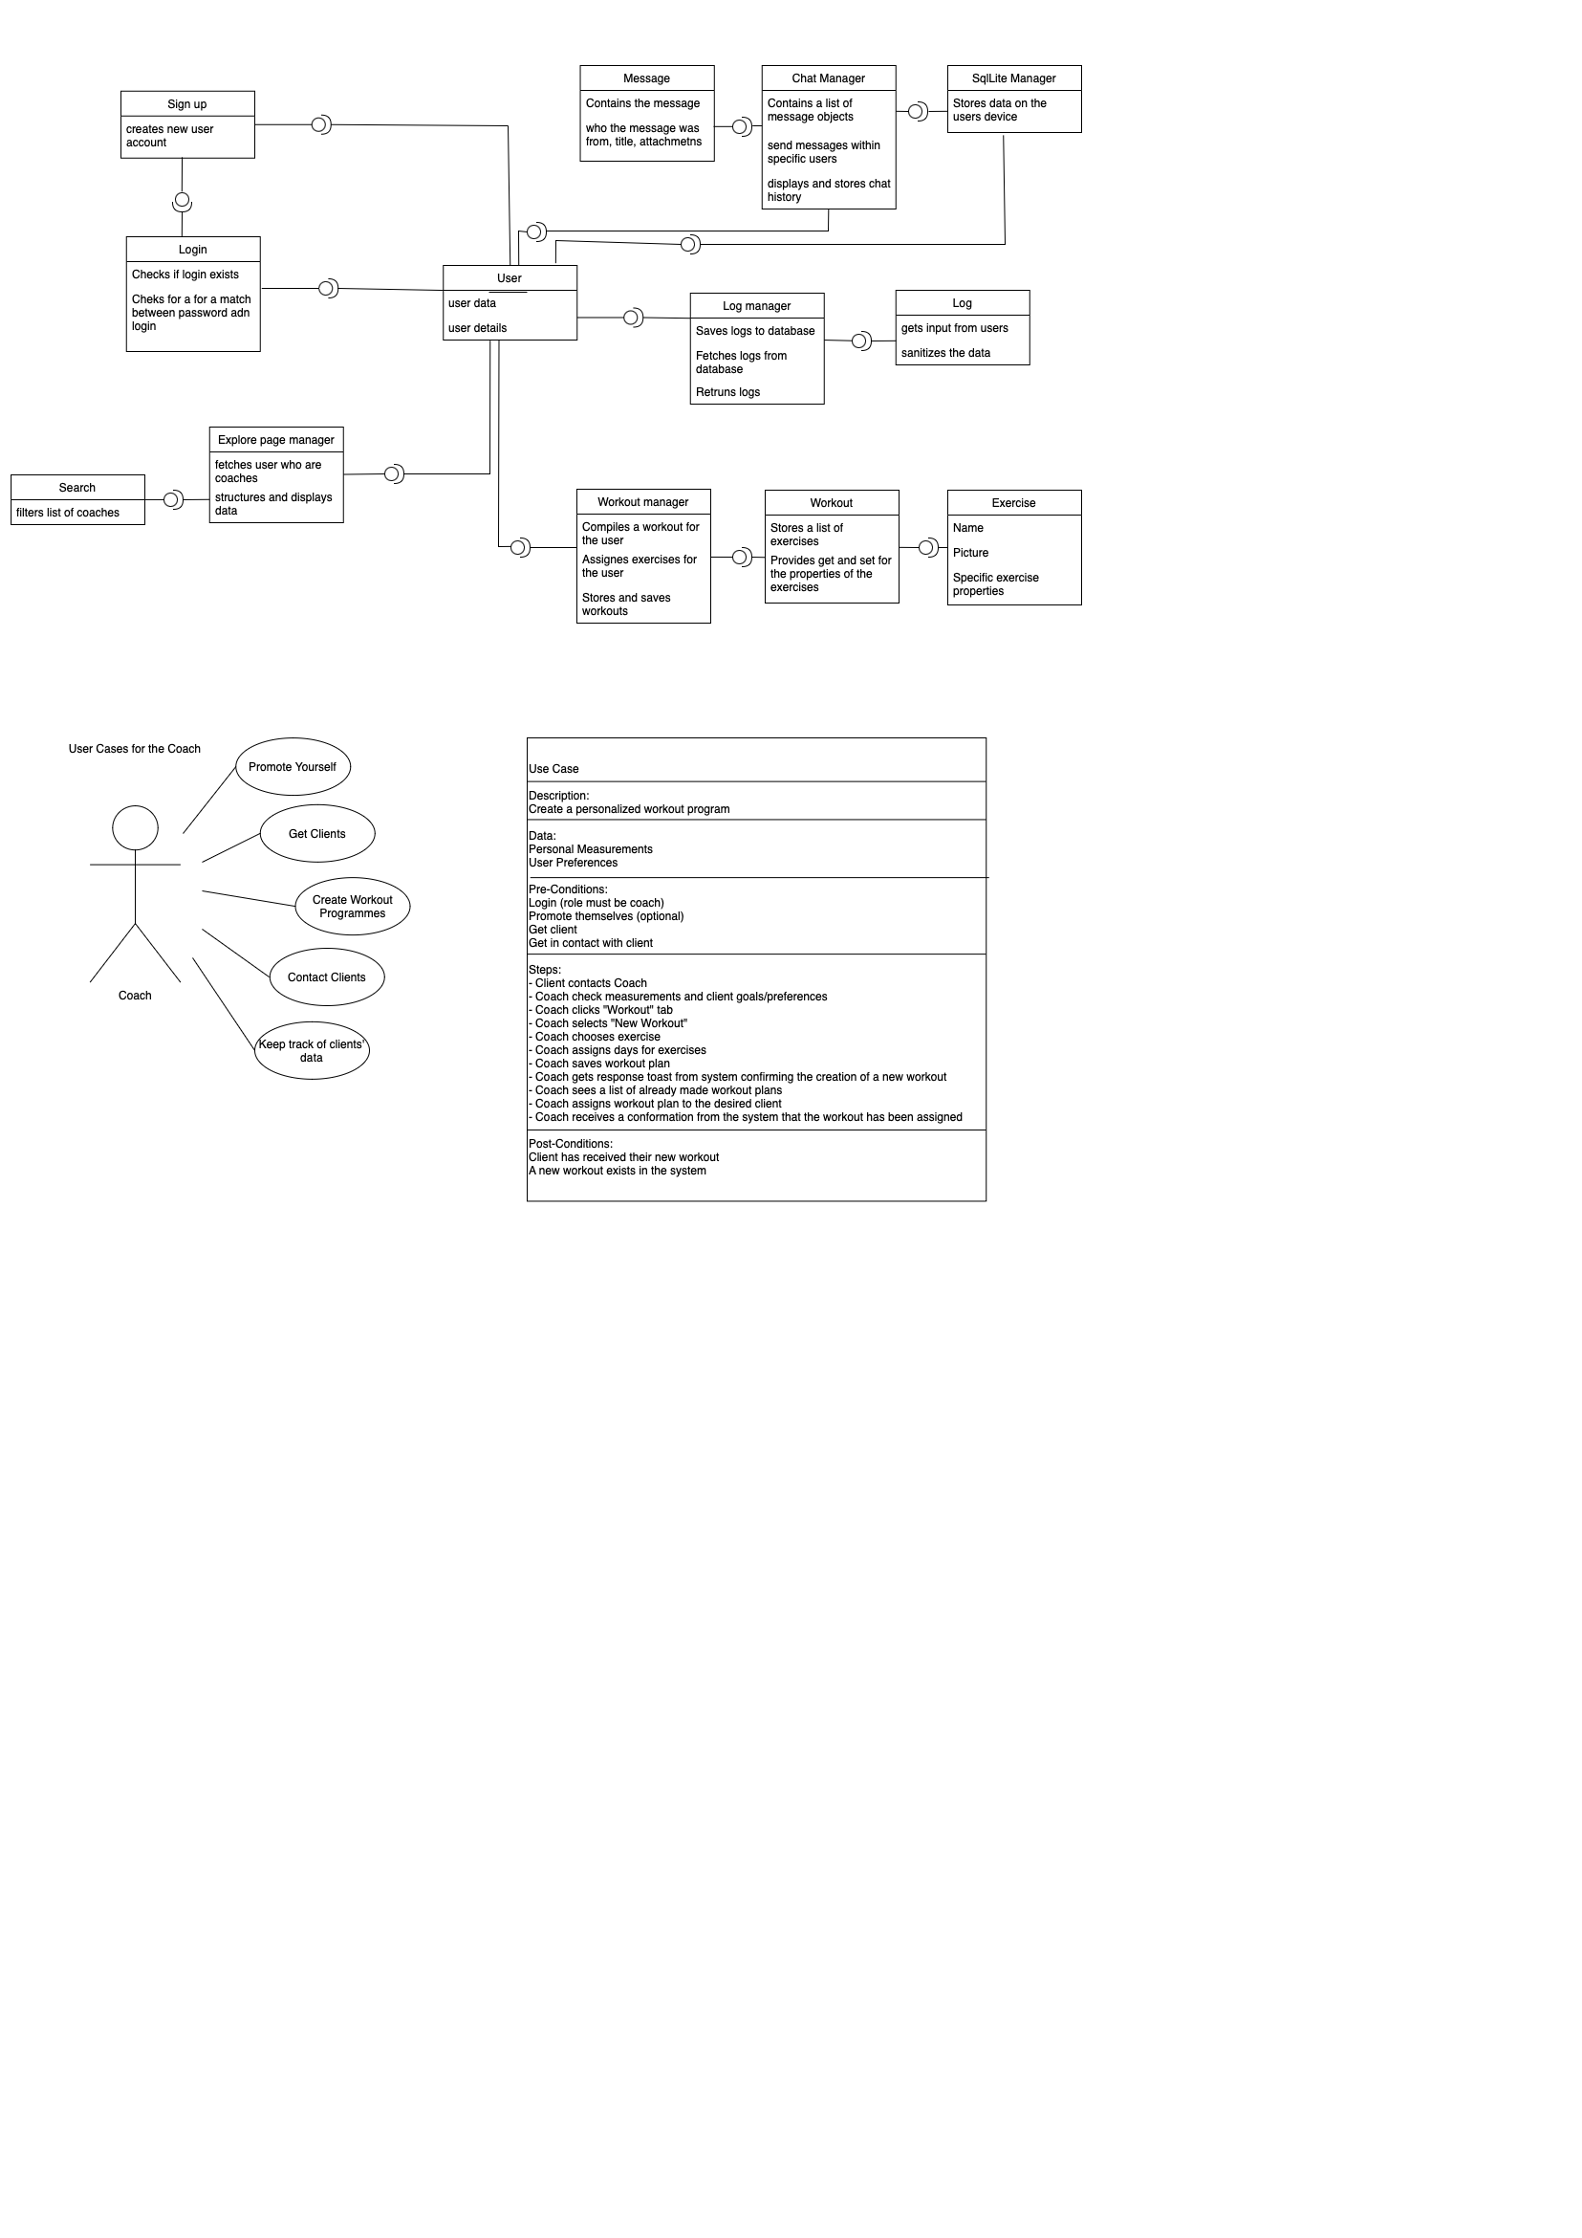
\includegraphics[width=0.8\textwidth]{images/usercase.png}
    \caption{ UML Diagram }
    \label{fig:usercase}
  \end{figure}

  \begin{figure}[H]
    \centering
    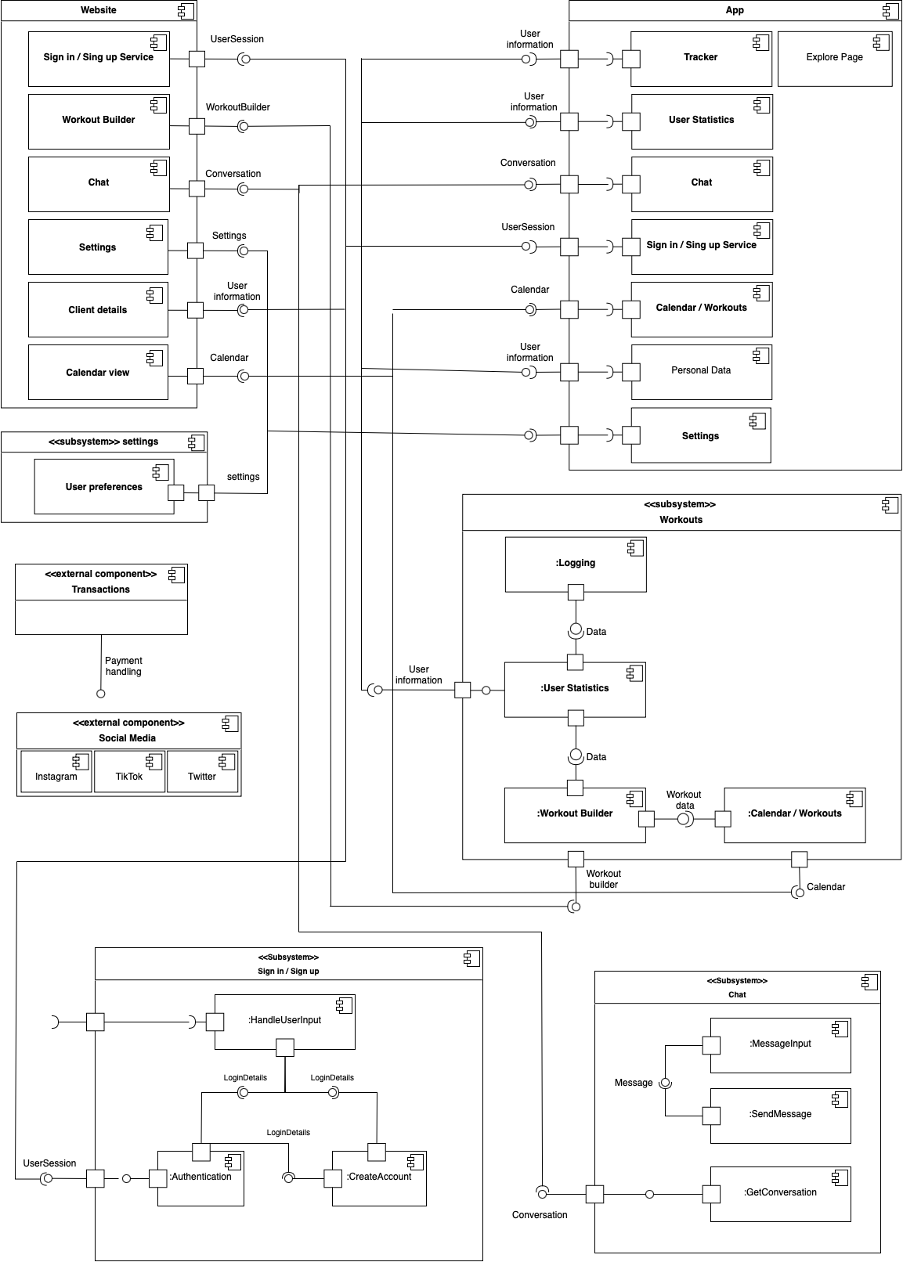
\includegraphics[width=0.8\textwidth]{images/component.png}
    \caption{ User Cases for Coach }
    \label{fig:component}
  \end{figure}



\subsection{Maintenance}
To ensure LinkedGym's reliability and longevity we also focused on effective maintenance. Our maintenance strategy includes:

\begin{itemize}
  \item \textbf{Continuous Integration/Continuous Deployment (CI/CD):} Implementing CI/CD pipelines to automate testing and deployment, ensuring seamless integration of updates and new features.
  
  \item \textbf{Monitoring and Logging:} Utilizing Firebase Performance Monitoring and Logging to track application performance, quickly identify issues, and maintain optimal user experience.
  
  \item \textbf{Regular Updates:} Delivering regular updates to fix bugs, introduce new features, and enhance existing functionalities based on user feedback and evolving market needs.

\begin{itemize}
\item \textbf{User Feedback:} Actively collecting and analyzing user feedback to drive continuous improvement and ensure the platform meets user needs and expectations.

\item \textbf{Comprehensive Documentation:} Maintaining detailed documentation for developers and users to facilitate smooth onboarding, usage, and troubleshooting.
\end{itemize}
\end{itemize}


\subsection{Conclusion}
The design phase of LinkedGym emphasizes a user-centric approach, agile development practices, and thorough planning. By leveraging a cloud-based architecture, detailed wireframes, and robust maintenance strategies, we aim to deliver a high-quality platform that meets the evolving needs of the fitness coaching industry. Our iterative approach ensures that we remain responsive to changes, deliver value consistently, and create a seamless and engaging user experience.
